\documentclass[a4paper,french,bookmarks]{article}

\usepackage[
    top         = 1in,
    bottom      = 1in,
    inner       = 1.5in,
    outer       = 1in,
    headheight  = 16pt,
    headsep     = 0.4in,
    footskip    = 0.4in,
    includeheadfoot,
    heightrounded,
    twoside,
    %showframe,
    ]{geometry}
\usepackage{booktabs}
\usepackage{minitoc}
\usepackage{./Structure/4PE18TEXTBnogeom}
\usepackage{proof}
\usepackage{pdfpages}
\usepackage[skip=10pt plus1pt,indent=40pt]{parskip}
\usepackage{blindtext}
\usepackage{biblatex}
\usepackage{svg}

\addbibresource{refs.bib}

\makeatletter
\renewcommand\tableofcontents{%
    \@starttoc{toc}%
}
%\renewcommand*\l@section{\@dottedtocline{1}{1em}{3em}}
\renewcommand*\l@subsection{\@dottedtocline{2}{2em}{3em}}
\makeatother

\newboxans
\renewcommand{\thesection}{\Roman{section}}
\renewcommand{\thesubsection}{\thesection.\arabic{subsection}}
\mtcsettitle{minitoc}{}

\DeclareDocumentCommand\Sp{g}{\funlv{Sp}{#1}}

\lstnewenvironment{outputlog}{
    \lstset{
        tabsize=2,
        breaklines,
        basicstyle=\footnotesize\ttfamily,
        frame=leftline
    }
}{}

\begin{document}
    
    %==============================
    % METADONNEES
    %==============================
    
    \title{}
    \author{SIAHAAN--GENSOLLEN Rémy}
    \date{\today}
    \hypersetup{
        pdftitle={Durcissement des villes modernes face aux rayonnements ionisants},
        pdfauthor={SIAHAAN--GENSOLLEN Rémy},
        pdflang={fr-FR},
        pdfsubject={Rapport de TIPE, Durcissement des villes modernes face aux rayonnements ionisants},
        pdfkeywords={TIPE, 2022-2023}
        pdfstartview=
    }
    
    %==============================
    % MISE EN PAGE
    %==============================

    %top         = 1.5in,
    %bottom      = 1.5in,
    %inner       = 1.5in,
    %outer       = 1in,
    %headheight  = 16pt,
    %headsep     = 0.3in,
    %footskip    = 0.3in,
    %includeheadfoot,
    %heightrounded,
    %twoside
    
    %==============================
    % STYLE DES EN-TÊTES ET PIEDS DE PAGES
    %==============================
    
    \fancypagestyle{plain}{
        \fancyhf{}
        \renewcommand{\headrulewidth}{0pt}
        \renewcommand{\footrulewidth}{0pt}
        \fancyfoot[RO,LE]{\sffamily\color{white5}\thepage~/~\pageref{LastPage}}
        %\fancyhead[LE]{\sffamily\color{white5}\bfseries SIAHAAN--GENSOLLEN Rémy}
        \fancyhead[LE]{\sffamily\color{white5}Rapport de TIPE}
        %\fancyhead[LO]{\sffamily\color{white5}\nouppercase{\rightmark}}
        \fancyhead[RO]{\sffamily\color{white5}Durcissement des villes modernes face aux rayonnements ionisants}
    }

    \pagestyle{plain}

    %==============================
    % CONTENU
    %==============================
    
    \begin{tcolorbox}[
            enhanced,
            frame hidden,
            sharp corners,
            spread upwards      = 0.1in,
            halign              = center,
            valign              = center,
            interior style      = {color=main3!20},
            arc                 = 0in,
            outer arc           = 0pt,
            leftrule            = 0pt,
            rightrule           = 0pt,
            fontupper           = \color{black},
            %width               = \paperwidth, 
            top                 = 0.4in, 
            bottom              = 0.3in
        ]
            {\large{\scshape{SIAHAAN--GENSOLLEN}} Rémy\par}
            \vspace{0.3in}
            {\Huge\sffamily{Rapport de TIPE}\par}
    	\vspace{0.05in}
            {\Huge\bfseries\sffamily Durcissement des villes modernes face aux rayonnements ionisants\par}
    \end{tcolorbox}

    \section*{Résumé}

    Les villes modernes regorgent de matériel électronique, et dépendent fortement de systèmes informatiques complexes. De par leur envergure, elles s'exposent grandement aux menaces des rayonnements ionisants. La question du durcissement des composants électroniques, particulièrement en de grandes concentrations, se pose donc dans le cadre de la résilience des villes. Dans ce TIPE, on se propose d'étudier dans un premier temps la sensibilité du matériel micro-technologique aux rayons ionisants et d'évaluer les risques de \emph{bit-flip} (inversion spontanée de la valeur d'un bit) à l'échelle d'une ville, puis dans un second de proposer différentes solutions de \emph{durcissement} pour palier ces problèmes.\bigskip
    
    \begin{tcolorbox}[
        enhanced,
        frame hidden,
        sharp corners,
        detach title,
        spread outwards,
        halign              = center,
            valign              = center,
        borderline west     = {3pt}{0pt}{main3},
        coltitle            = main3, 
        interior style      = {
            left color      = main1white2!65!gray!11,
            middle color    = main1white2!50!gray!10,
            right color     = main1white2!35!gray!9
        },
        arc                 = 0 cm,
        title               = SOMMAIRE,
        boxrule             = 0pt,
        fonttitle           = \bfseries\sffamily,
        overlay             = {
            \node[rotate=90, minimum width=1cm, anchor=south,yshift=-0.8cm]
            at (frame.west) {\tcbtitle};
        },
    ]
        \begin{minipage}{0.83\linewidth}
            \sffamily
            \tableofcontents
        \end{minipage}
    \end{tcolorbox}

    \bigskip

    \section{Présentation du problème}

    \subsection{Motivations}

    La municipalité de Schaerbeek, en Belgique, lors des élections législatives du 18 mai 2003, a été le théâtre d'une scène particulière : une des machines utilisées pour comptabiliser les votes affichait, pour l'un des candidats, un nombre supérieur de $4096$ voix par rapport au compte manuel. Comme ce nombre peut le suggérer, l'explication retenue par les autorités après analyse de la machine est que l'inversion spontanée de la valeur d'un bit dans la mémoire vive de la machine, à la 13\ieme position, a attribué ces $2^{12}$ votes supplémentaires \cite{nappa2021dejavu}. 

    Dans le monde du jeu vidéo, les \guill{speedrunners} sont une catégorie des joueurs cherchant à atteindre un objectif donné (par exemple terminer le jeu) le plus rapidement possible. En 2013, l'un d'entre eux rencontre un bug étrange sur \emph{Super Mario 64}, un des jeux les plus prisé par cette communauté : il est soudainement téléporté sur un niveau supérieur, lui faisant gagner un temps précieux. Très vite, la communauté cherche à reproduire le bug, et l'on propose même une récompense de $1000~\$$ pour qui y parviendra. Pourtant, même en simulant exactement les même mouvements que le joueur, on ne parvient pas à le reproduire. Cette fois aussi, l'explication qui donne le résultat le plus convaincant est l'inversion spontanée de la valeur d'un bit :
    %
    \[ \text{Hauteur de Mario dans le jeu :}\qquad \underbrace{C5\!}_{\makebox[0pt]{\small 1100010\colorbox{main3!85!gray!20}{\color{main3}\bfseries 1}}}\!837800 \ \xlongrightarrow{\text{inversion spontannée}} \ \underbrace{C4\!}_{\makebox[0pt]{\small 1100010\colorbox{main3!85!gray!20}{\color{main3}\bfseries 0}}}\!837800 \]
    %
    En simulant artificiellement ce changement, on obtient une scène très proche de l'originale \cite{burtt20}. 

    Des situations similaires aux deux présentées ci-dessus se produisent régulièrement, de partout sur la planète. Ce phénomène est généralement nommé \emph{erreur logicielle}, \emph{soft fail} ou \emph{soft error}, et est difficilement reproductible. Plus précisément, \textsc{Ziegler} et \textsc{Lanford} donnent dans un article de 1979 \cite{ziegler79} la définition suivante :
    
    \begin{definition}{Soft-fail}{}
        On appelle \hg{soft-fail} l'inversion spontanée de la valeur d'un bit (\hg{bit-flip}), lequel fonctionnera correctement lorsqu'il sera testé plus tard.
    \end{definition}
    
    Les soft-fails sont principalement considérés comme étant dus aux rayons ionisants \cite{ziegler96,ziegler79}. Ces derniers, découverts à la fin du \textsc{XIX}\ieme siècle (à peu près au même moment que la radioactivité), sont toujours étudiés aujourd'hui : le \emph{Comité scientifique des Nations Unies pour l'étude des effets des rayonnements ionisants}, ou UNSCEAR en anglais, est chargé depuis sa fondation en 1955 d'examiner les sources de rayonnements ionisants et leurs effets sur la santé humaine et l'environnement. En effet, une trop grande exposition aux rayons ionisants peut causer des lésions des tissus biologiques, endommager l'ADN, résulter en l'apparition de pathologies et cancers, et ainsi même entraîner la mort de l'individu \cite{UNSCEAR08}. On en donne la définition suivante :
    
    \begin{definition}{Rayonnement ionisant}{}
        On appelle \hg{rayonnement ionisant} un transport d'énergie sous forme de particules subatomiques ou d'ondes électromagnétiques de forte fréquence, ayant une énergie suffisante pour arracher des électrons aux atomes qu'ils traversent.
    \end{definition}
    
    Le rapport de l'UNSCEAR de 2008 \cite{UNSCEAR08} détaille les nombreuses sources de ces radiations. Si certains rayonnements sont d'origine humaine (tests nucléaires, appareils médicaux), d'autres sont d'origine naturelle \cite{nappa2021dejavu,UNSCEAR08,ziegler96,ziegler79,ziegler81}: rayons cosmiques, ceintures de radiation de \textsc{Van Allen}, rayonnement terrestre, ... Au delà des soft-fails, les rayons ionisants sont également susceptibles de réarranger les cristaux utilisés dans les composants et de les endommager définitivement et causer des dommages permanents (on parle alors d'\emph{erreur matérielle} ou de \emph{hard-fail}).

    Les rayons cosmiques notamment, découverts en 1913, ont posé de nombreux problèmes au bon fonctionnement des composants électroniques embarqués dans les satellites ou les avions \cite{ziegler96, nappa2021dejavu}. Une grande partie de ces particules, les plus énergétiques et les plus dangereuses, rentre en collision avec la matière de l'atmosphère avant d'atteindre le sol, mais la partie qui y parvient pose problème au matériel de haute technologie. Si jusqu'ici les rayons ionisants touchaient dans une majorité statistique de cas des régions non allouées de mémoire, les nouvelles générations de composants utilisant des circuits de bien plus petites tailles y sont de plus en plus sensibles et s'exposent à d'importants risques de soft-fails \cite{ziegler96, ziegler79, ziegler81}.

    Les villes modernes regroupant de grandes densités de matériel électronique de pointe et de systèmes informatiques interdépendants, elles sont donc particulièrement menacées par les radiations ionisantes. \textsc{Nappa}, \textsc{Hobbs} et \textsc{Lanzi} discutent par exemple en 2021 \cite{nappa2021dejavu} la possibilité de déverrouiller un téléphone en utilisant des rayonnements ionisants pour inverser la valeur de certai   ns bits dans la mémoire et causer des erreurs de segmentation. Enfin, les rayonnements ionisants sont une grande menace à la stabilité des futurs ordinateurs quantiques \cite{nappa2021dejavu}, qui seront probablement employés dans les villes du futur. On cherchera donc de quantifier le phénomène (fréquence des rayons cosmiques à hauteur des villes et des soft-fails), et à proposer des solutions pour palier les problèmes causés, dites de \emph{durcissement}.

    \subsection{Approche expérimentale}

    Une première idée a d'abord été de se munir d'un disque dur \guill{relativement vieux}, qui serait similaire à ceux des situations présentées ci-dessus. Après quelques recherches, j'ai réussi à me procurer un disque \emph{Barracuda 7200.8 Serial ATA}, modèle \texttt{ST3250823AS} de \textsf{SeaGate\textsuperscript{\tiny\textregistered}} de 2007, d'une capacité de $\qty{250}{\giga\byte}$. Une photographie et les dimensions en sont données sur les figures \ref{fig:fig1} et \ref{fig:fig2} ci-dessous :
    %
    \begin{center}
        \begin{minipage}{0.4\linewidth}
            \begin{center}
                \includegraphics[scale=0.4]{../Images/disqueTIPEphoto.png}
                
                \captionof{figure}{Photographie du disque}
                \label{fig:fig1}
            \end{center}
        \end{minipage}
        %
        \begin{minipage}{0.1\linewidth}
            \hfill
        \end{minipage}
        %
        \begin{minipage}{0.4\linewidth}
            \begin{center}
                \begin{tikzpicture}
                    \node[anchor=south west,inner sep=0] at (0,0) {\includesvg[width = 0.9\textwidth]{../Images/disque.svg}};
    
                    \draw[<->] (0, 2) --node[midway,above, sloped, align=center] {$\qty{146.9898}{\mm}$} (3, 3.75);
    
                    \draw[<->] (3.2, 3.8) --node[midway,above, sloped, align=center] {$\qty{101.6}{\mm}$} (5.3, 2.6);
    
                    \draw[<->] (5.5, 2.4) --node[midway,above, sloped, align=center] {$\qty{26.111}{\mm}$} (5.5, 1.6);
                \end{tikzpicture}
    
                \captionof{figure}{Dimensions du disque}
                \label{fig:fig2}
            \end{center}
        \end{minipage}
    \end{center}
    %
    En connectant le disque à un ordinateur sous un système d'exploitation (ici \textsf{Debian}), on peut grâce à la commande Unix \texttt{dd} afficher le contenu du périphérique (ici \texttt{/dev/sda}), spécifié par l'argument \texttt{if}. On peut ensuite pipe le résultat avec la commande \texttt{hd} pour afficher le contenu en hexadecimal puis \texttt{less} pour afficher le détail progressivement. En résumé, on a :
    %
    \begin{bash}
dd if=/dev/sda | hd | less
    \end{bash}
    %
    \begin{outputlog}
00000000  33 c0 fa 8e d8 8e d0 bc  00 7c 89 e6 06 57 8e c0  |3........|...W..|
00000010  fb fc bf 00 06 b9 00 01  f3 a5 ea 1f 06 00 00 52  |...............R|
00000020  52 b4 41 bb aa 55 31 c9  30 f6 f9 cd 13 72 13 81  |R.A..U1.0....r..|
00000030  fb 55 aa 75 0d d1 e9 73  09 66 c7 06 8d 06 b4 42  |.U.u...s.f.....B|
00000040  eb 15 5a b4 08 cd 13 83  e1 3f 51 0f b6 c6 40 f7  |..Z......?Q...@.|
00000050  e1 52 50 66 31 c0 66 99  e8 66 00 e8 35 01 4d 69  |.RPf1.f..f..5.Mi|
00000060  73 73 69 6e 67 20 6f 70  65 72 61 74 69 6e 67 20  |ssing operating |
00000070  73 79 73 74 65 6d 2e 0d  0a 66 60 66 31 d2 bb 00  |system...f`f1...|
00000080  7c 66 52 66 50 06 53 6a  01 6a 10 89 e6 66 f7 36  ||fRfP.Sj.j...f.6|
00000090  f4 7b c0 e4 06 88 e1 88  c5 92 f6 36 f8 7b 88 c6  |.{.........6.{..|
...
    \end{outputlog}
    %
    \noindent On peut alors ré-écrire la totalité du disque pour qu'il n'y ait que des zéros, en utilisant le pseudo-périphérique \texttt{/dev/zero} (qui renvoie le caractère nul), et le paramètre \texttt{bs=16M} pour augmenter la taille du buffer (ce qui accélère grandement la manipulation) :
    %
    \begin{bash}
dd if=/dev/zero of=/dev/sda bs=32M
    \end{bash}
    %
    \begin{outputlog}
00000000  00 00 00 00 00 00 00 00  00 00 00 00 00 00 00 00  |................|
*
f196b000
    \end{outputlog}
    %
    On observe bien que le contenu du disque a entièrement été remplacé par des zéros. La praticité de cet affichage est que toutes les lignes identiques (ici des lignes de zéros) sont résumées avec le symbole \texttt{*}. Ainsi, un bit-flip sera facile à repérer, la ligne apparaissant directement. On peut alors démonter la partie métallique autour du disque, et laisser pendant plusieurs semaines le disque exposé. Malheureusement, même après huit semaines d'expérimentation, aucun bit-flip n'est constaté sur le disque. Cet échec peut s'expliquer par plusieurs facteurs :
    %
    \begin{enumerate}
        \ithand les \guill{vieux} disques comme celui utilisé ont des composants de plus grande taille et sont moins sensibles aux rayons ionisants ;

        \ithand il peut déjà y avoir des mécanisme de durcissement, matériel notamment ;

        \ithand si le phénomène est trop rare, un seul disque exposé pendant huit semaines peut ne pas être suffisant.
    \end{enumerate}
    %
    \noindent On notera d'ailleurs que les rayons cosmiques sont plus présent à haute altitude qu'au niveau de la mer \cite{ziegler96}, on aurait donc pu avoir plus de résultat à la montagne par exemple qu'à Paris où l'expérience a été réalisée (altitude de $\qty{35}{\meter}$).

    \subsection{Données réelles et modélisation}

    Faute de pouvoir mesurer expérimentalement la fréquence des soft-fails, on peut utiliser les données fournies dans la littérature. En ce qui concerne le point abordé précédemment à propos de l'altitude, le rapport 2008 de l'UNSCEAR \cite{UNSCEAR08} fournit la figure \ref{fig:fig3} ci-dessous, où la dose équivalente désigne une grandeur caractérisant l'impact sur le corps des rayonnements ionisants.
    %
    \begin{center}
        
        \begin{minipage}{0.4\linewidth}
            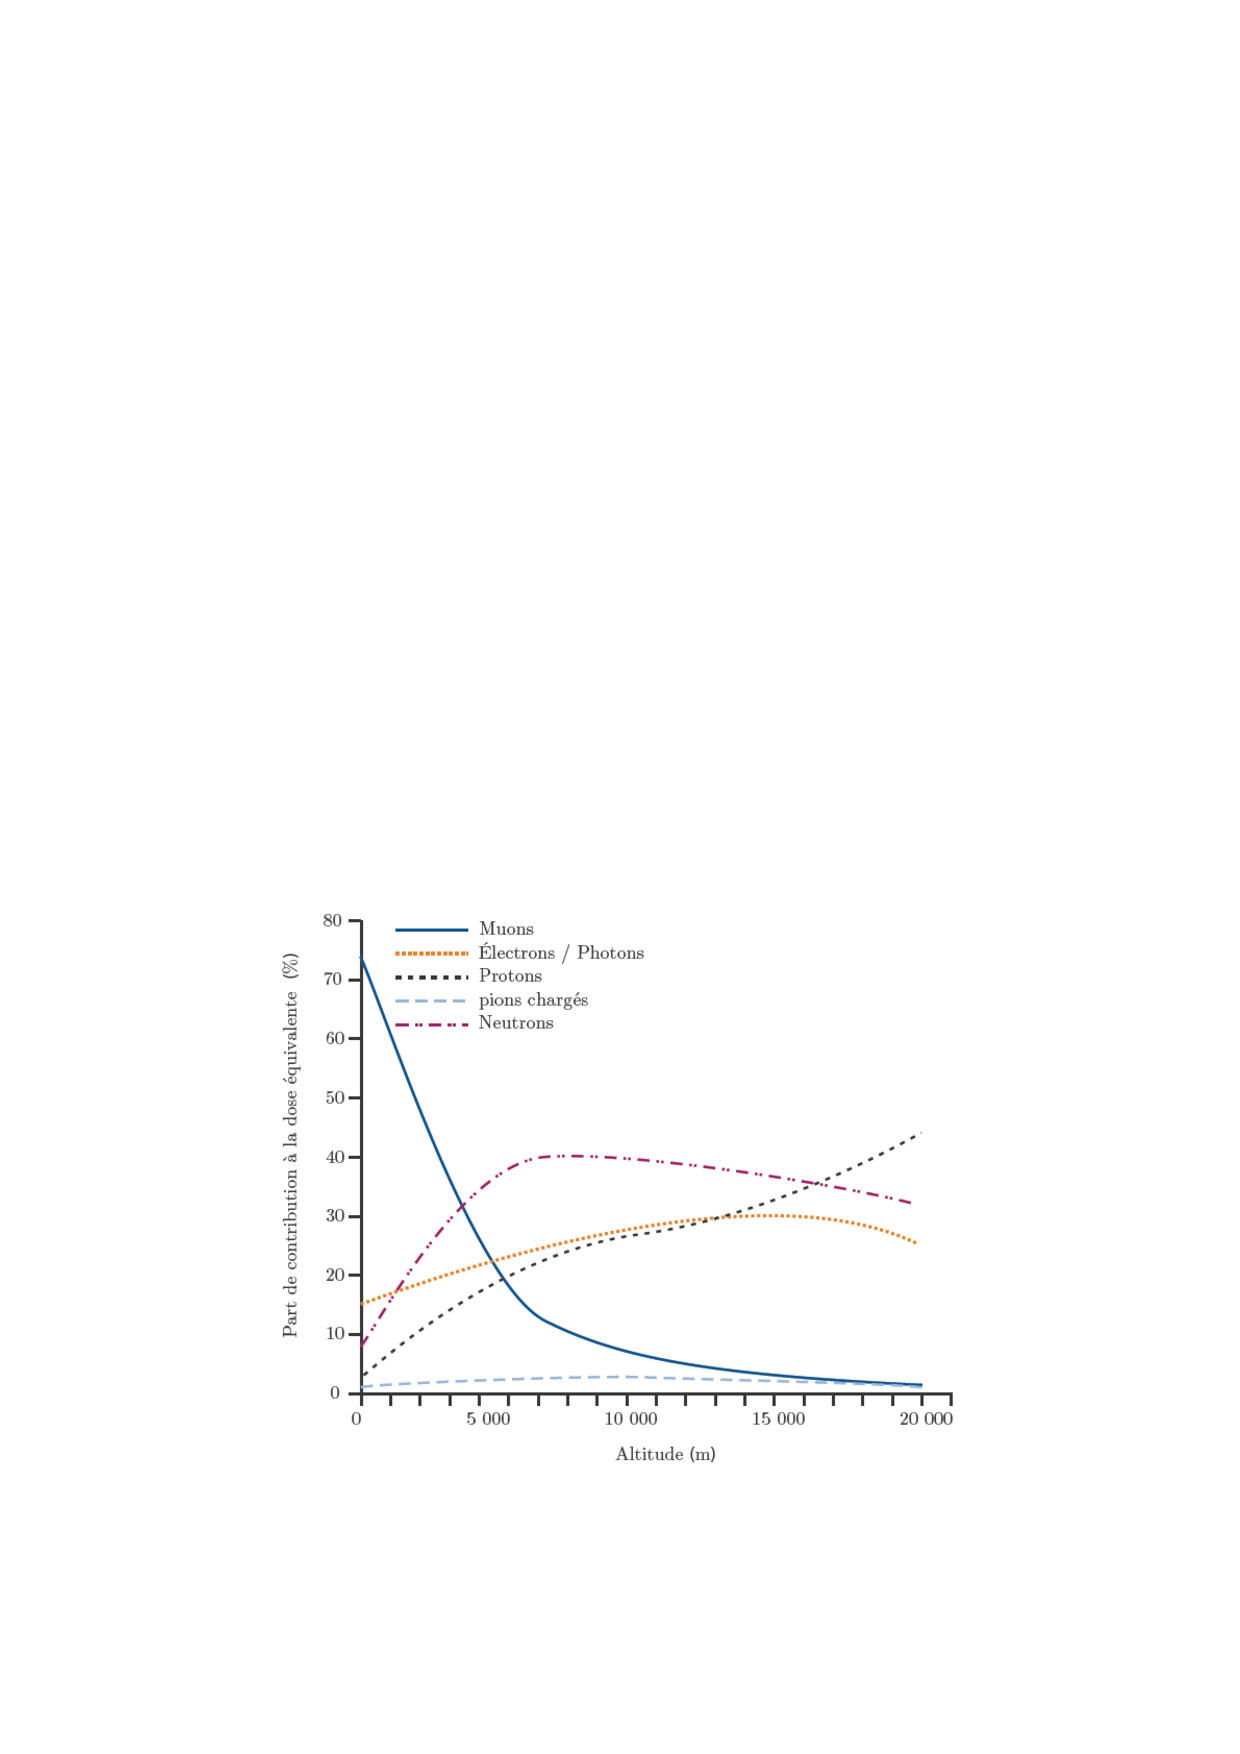
\includegraphics[scale=0.6]{../Images/unscear2008cosmic.pdf}
            \captionof{figure}{Part de contribution des rayons cosmiques à la dose équivalente en fonction de l'altitude}
            \label{fig:fig3}
        \end{minipage}
        %
        \begin{minipage}{0.1\linewidth}
            \hfill
        \end{minipage}
        %
        \begin{minipage}{0.4\linewidth}
            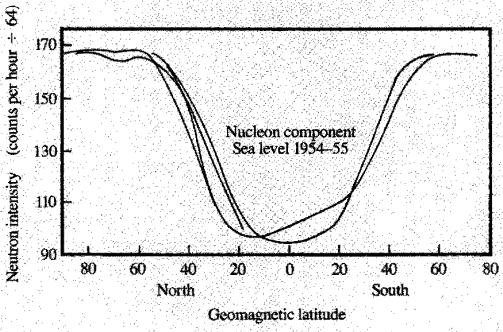
\includegraphics[scale=0.6]{../Images/latitude.png}

            \captionof{figure}{Exposition aux rayons cosmiques en fonction de la latitude magnétique}
            \label{fig:fig4}
        \end{minipage}
        
        
    \end{center}
    %
    On observe que les particules les plus énergétiques comme les protons ou les neutrons sont plus présent à haute altitude\cite{nappa2021dejavu, ziegler96}. C'est donc notamment un critère à prendre en compte pour déterminer la sensibilité d'une ville aux rayons ionisants. Un autre critère similaire est celui de la position de la ville sur Terre. Plus précisément, la latitude géomagnétique (définie de manière similaire à la latitude géographique) est déterminante dans l'exposition aux rayons cosmiques : \textsc{Ziegler} montre en 1996 (\cf. figure \ref{fig:fig4}) que les pôles sont environ deux fois plus exposés que l'équateur \cite{ziegler96}.

    À partir des données sur la quantité de rayons ionisants, il est possible de construire un modèle théorique pour estimer les taux de soft-fails. Ainsi, \textsc{Ziegler} et \textsc{Lanford} établissent dans leur article de 1981 \cite{ziegler81} qu'un semi-conducteur de l'époque de $\qty{10}{\micro\meter\squared}$ est sujet à environ un soft-fail par jour.
    
    \section{Solutions de durcissement}

    \subsection{Durcissement matériel}

    Pour protéger le matériel de haute de technologie, et donc les villes, de tels dysfonctionnements, on a recours à un ensemble de techniques interdisciplinaires \cite{mittal16}, ce qu'on appelle \emph{durcissement (électronique)}, ou \emph{radiation hardening} (les composants sont alors qualifiés de \emph{radio-durcis} ou de \emph{rad-hard}).
    
    Une première solution est de protéger physiquement les données, ce qu'on appelle \emph{durcissement matériel}. Pour cela on peut, au lieu d'utiliser les matériaux semi-conducteurs classique, utiliser un substrat isolant comme l'oxyde d'aluminium ou de silicium. On parle respectivement des technologies \emph{Silicon On Saphire} (abrégé \emph{SOS}) et \emph{Silicon On Insulator})\cite{mittal16, shunkov20}. D'autres méthodes consistent à blinder les composants dans des boîters résistant aux radiations. Toutefois de telles techniques, même si elles démontrent une efficacité certaine, ne sont pas infaillibles et les risque de soft-fail pour les composants ne sont pas réduits à zéro.

    \subsection{Durcissement logique : codes correcteurs}

    Plutôt que de passer par un durcissement matériel, on peut proposer des solutions algorithmiques : l'idée générale est de rendre l'information redondante (de manière optimale) pour qu'en cas de soft-fail l'information ne soit pas corrompue. Une branche des mathématique et de l'informatique, celle des \emph{codes correcteurs}, se penche sur cette problématique.

    \subsection{Durcissement logique : cas de la technologie RAID}

    Inventée en 1986, la technologie \textsf{RAID} (pour \emph{Redundant Arrays of Inexpensive Disks}, soit \emph{regroupement redondant de disques peu coûteux} en français) permet de répartir des données sur plusieurs disques durs, et peut servir notamment à améliorer la sécurité de l'information stockée face à la perte d'un disque. Le niveau appelé \textsf{RAID-6} permet de rendre l'information $n$ fois redondante, et supporte donc la perte de jusqu'à $n$ disques. Les principes théoriques derrière cette technologie, on se limitera ici au cas $n = 2$. 
    
    On commence par se placer dans l'ensemble fini $\bdF_{256} = \iint{0, 255} = \iint{0, 2^8 - 1}$. On représente tout élément de cet ensemble sous base hexadécimale avec la notation $\ens{xy} = 15x + y$. On écrit également $n_i$ le $i$\ieme bit en partant de la droite dans l'écriture en binaire de $n$ (pour $i \in \iint{0, 7}$). Par exemple, pour $n = 94 \in \bdF_{256}$, on a $n = \ens{5e}$, et en binaire $n = \overline{01011110}^2$ donc $n_7 = n_5 = n_0 = 0$ et $n_6 = n_4 = n_3 = n_2 = n_1 = 1$. On munit alors $\bdF_{256}$ des opérations suivantes :
    %
    \begin{enumerate}
        \itt Une \guill{addition} $\oplus$ qui est un ou exclusif sur chaque bit : $\p{n \oplus n'}_i = \begin{cases}
            1 &\text{si } n_i + n_i' = 1\\
            0 &\text{sinon}
        \end{cases}$.

        Cette loi possède un élément neutre, à savoir $0$, et tout élément $n \in \bdF_{256}$ est son propre inverse par cette loi (on a $n \oplus n = 0$). Elle est également commutative et associative. 

        \itt Une multiplication $\times$ définie de sorte que pour $n \in \bdF_{256}$ :
        %
        \[ n \times 0 = 0\qquad n \times 1 = n \qquad \begin{cases}\p{n \times 2}_0 = n_7\\
        \p{n \times 2}_1 = n_0\\
        \p{n \times 2}_2 = n_1 + n_7\\
        \p{n \times 2}_3 = n_2 + n_7\\
        \p{n \times 2}_4 = n_3 + n_7\\
        \p{n \times 2}_5 = n_4\\
        \p{n \times 2}_6 = n_5\\
        \p{n \times 2}_7 = n_6
        \end{cases}\]
        %
        Et telle qu'elle soit associative, commutative, et distributive sur $\oplus$. Pour tout $n \in \bdF_{256} \backslash 0$, on peut alors montrer qu'il existe $n' \in \bdF_{256}$ tel que $n \times n' = 1$.
    \end{enumerate}
    %
    Cette multiplication peut être implémentée avec le code suivant, à l'aide des opérations par bits :
    %
    \begin{C}
uint8_t c, cc;
cc = (c << 1) ^ ((c & 0x80) ? 0x1d : 0);
    \end{C}
    %
    En bref, $\bdF_{256}$ est un corps (il s'agit en fait de l'unique corps fini à $256$ éléments, aussi appelé \emph{corps de \textsc{Galois} $\bbG\bbF\p{256}$}).

    On peut alors considérer $n \leq 255$ disques, représentés par des vecteurs $u_1, u_2, \dots, u_n$ de valeurs de $\bdF_{256}$, et calculer, pour un générateur $g$ du corps (par exemple $g = 2$) :
    %
    \[ p = u_1 \oplus u_2 \oplus \dots \oplus u_{n-1} \qquad\et\qquad q = g^0 \times u_0 \oplus g^1 \times u_1 \oplus \dots g^{n-1} \times D^{n-1} \]
    %
    Le vecteur $q$ est appelé code de \textsc{Reed-Solomon}. Si on perd un des disques $u_i$, le vecteur $p$ permet par opération XOR de retrouver le vecteur. Si l'on perd $p$ ou $q$, on peut simplement les recalculer.

    Si on perd un $u_i$ et $q$, de même. Si l'on perd un $u_i$ et $p$, on peut calculer $q_x$
    %
    \[ q_x = q + g^x \cdot D_x\]

    \newpage
    

    %Un premier cas est celui de \textsf{RAID-5} qui fonctionne en redondance $n + 1$ : chaque disque est découpé en \guill{bandes}, 

    \printbibliography[heading=bibintoc,title={Bibliographie}]

\end{document}